%%% The main file. It contains definitions of basic parameters and includes all other parts.

%% Settings for single-side (simplex) printing
% Margins: left 40mm, right 25mm, top and bottom 25mm
% (but beware, LaTeX adds 1in implicitly)
\documentclass[12pt,a4paper]{report}
\setlength\textwidth{145mm}
\setlength\textheight{247mm}
\setlength\oddsidemargin{15mm}
\setlength\evensidemargin{15mm}
\setlength\topmargin{0mm}
\setlength\headsep{0mm}
\setlength\headheight{0mm}
% \openright makes the following text appear on a right-hand page
\let\openright=\clearpage

%% Settings for two-sided (duplex) printing
% \documentclass[12pt,a4paper,twoside,openright]{report}
% \setlength\textwidth{145mm}
% \setlength\textheight{247mm}
% \setlength\oddsidemargin{14.2mm}
% \setlength\evensidemargin{0mm}
% \setlength\topmargin{0mm}
% \setlength\headsep{0mm}
% \setlength\headheight{0mm}
% \let\openright=\cleardoublepage

%% Generate PDF/A-2u
\usepackage[a-2u]{pdfx}

%% Character encoding: usually latin2, cp1250 or utf8:
\usepackage[utf8]{inputenc}

%% Prefer Latin Modern fonts
\usepackage{lmodern}

%% Further useful packages (included in most LaTeX distributions)
\usepackage{amsmath}        % extensions for typesetting of math
\usepackage{amsfonts}       % math fonts
\usepackage{amsthm}         % theorems, definitions, etc.
\usepackage{bbding}         % various symbols (squares, asterisks, scissors, ...)
\usepackage{bm}             % boldface symbols (\bm)
\usepackage{graphicx}       % embedding of pictures
\usepackage{fancyvrb}       % improved verbatim environment
\usepackage[square,numbers]{natbib}         % citation style AUTHOR (YEAR), or AUTHOR [NUMBER]

\usepackage[nottoc]{tocbibind} % makes sure that bibliography and the lists
			    % of figures/tables are included in the table
			    % of contents
\usepackage{dcolumn}        % improved alignment of table columns
\usepackage{booktabs}       % improved horizontal lines in tables
\usepackage{paralist}       % improved enumerate and itemize
\usepackage{xcolor}         % typesetting in color
\usepackage{float}
\usepackage{listings}
\usepackage{color}
\usepackage{multirow}
\usepackage{subcaption}
%%% Basic information on the thesis

% Thesis title in English (exactly as in the formal assignment)
\def\ThesisTitle{A Methodical Approach to the Evaluation of Appearance Computations}

% Author of the thesis
\def\ThesisAuthor{Bc. Marcel Hruška}

% Year when the thesis is submitted
\def\YearSubmitted{2020}

% Name of the department or institute, where the work was officially assigned
% (according to the Organizational Structure of MFF UK in English,
% or a full name of a department outside MFF)
\def\Department{Department of Software and Computer Science Education}

% Is it a department (katedra), or an institute (ústav)?
\def\DeptType{Department}

% Thesis supervisor: name, surname and titles
\def\Supervisor{doc. Alexander Wilkie, Dr.}

% Supervisor's department (again according to Organizational structure of MFF)
\def\SupervisorsDepartment{Department of Software and Computer Science Education}

% Study programme and specialization
\def\StudyProgramme{Computer Science}
\def\StudyBranch{Computer Graphics and Game Development}

% An optional dedication: you can thank whomever you wish (your supervisor,
% consultant, a person who lent the software, etc.)
\def\Dedication{%
Dedication.
}

% Abstract (recommended length around 80-200 words; this is not a copy of your thesis assignment!)
\def\Abstract{%
Abstract.
}

% 3 to 5 keywords (recommended), each enclosed in curly braces
\def\Keywords{%
{key} {words}
}

%% The hyperref package for clickable links in PDF and also for storing
%% metadata to PDF (including the table of contents).
%% Most settings are pre-set by the pdfx package.
\hypersetup{unicode}
\hypersetup{breaklinks=true}

% Definitions of macros (see description inside)
%%% This file contains definitions of various useful macros and environments %%%
%%% Please add more macros here instead of cluttering other files with them. %%%

%%% Minor tweaks of style

% These macros employ a little dirty trick to convince LaTeX to typeset
% chapter headings sanely, without lots of empty space above them.
% Feel free to ignore.
\makeatletter
\def\@makechapterhead#1{
  {\parindent \z@ \raggedright \normalfont
   \Huge\bfseries \thechapter. #1
   \par\nobreak
   \vskip 20\p@
}}
\def\@makeschapterhead#1{
  {\parindent \z@ \raggedright \normalfont
   \Huge\bfseries #1
   \par\nobreak
   \vskip 20\p@
}}
\makeatother

% This macro defines a chapter, which is not numbered, but is included
% in the table of contents.
\def\chapwithtoc#1{
\chapter*{#1}
\addcontentsline{toc}{chapter}{#1}
}

% Draw black "slugs" whenever a line overflows, so that we can spot it easily.
\overfullrule=1mm

%%% Macros for definitions, theorems, claims, examples, ... (requires amsthm package)

\theoremstyle{plain}
\newtheorem{thm}{Theorem}
\newtheorem{lemma}[thm]{Lemma}
\newtheorem{claim}[thm]{Claim}

\theoremstyle{plain}
\newtheorem{defn}{Definition}

\theoremstyle{remark}
\newtheorem*{cor}{Corollary}
\newtheorem*{rem}{Remark}
\newtheorem*{example}{Example}

%%% An environment for proofs

\newenvironment{myproof}{
  \par\medskip\noindent
  \textit{Proof}.
}{
\newline
\rightline{$\qedsymbol$}
}

%%% An environment for typesetting of program code and input/output
%%% of programs. (Requires the fancyvrb package -- fancy verbatim.)

\DefineVerbatimEnvironment{code}{Verbatim}{fontsize=\small, frame=single}

%%% The field of all real and natural numbers
\newcommand{\R}{\mathbb{R}}
\newcommand{\N}{\mathbb{N}}

%%% Useful operators for statistics and probability
\DeclareMathOperator{\pr}{\textsf{P}}
\DeclareMathOperator{\E}{\textsf{E}\,}
\DeclareMathOperator{\var}{\textrm{var}}
\DeclareMathOperator{\sd}{\textrm{sd}}

%%% Transposition of a vector/matrix
\newcommand{\T}[1]{#1^\top}

%%% Various math goodies
\newcommand{\goto}{\rightarrow}
\newcommand{\gotop}{\stackrel{P}{\longrightarrow}}
\newcommand{\maon}[1]{o(n^{#1})}
\newcommand{\abs}[1]{\left|{#1}\right|}
\newcommand{\dint}{\int_0^\tau\!\!\int_0^\tau}
\newcommand{\isqr}[1]{\frac{1}{\sqrt{#1}}}

%%% Various table goodies
\newcommand{\pulrad}[1]{\raisebox{1.5ex}[0pt]{#1}}
\newcommand{\mc}[1]{\multicolumn{1}{c}{#1}}


% Title page and various mandatory informational pages
\begin{document}
%%% Title page of the thesis and other mandatory pages

%%% Title page of the thesis

\pagestyle{empty}
\hypersetup{pageanchor=false}
\begin{center}

\centerline{\mbox{
\includegraphics[width=166mm]{img/logo-en.pdf}}}

\vspace{-8mm}
\vfill

{\bf\Large MASTER THESIS}

\vfill

{\LARGE\ThesisAuthor}

\vspace{15mm}

{\LARGE\bfseries\ThesisTitle}

\vfill

\Department

\vfill

{
\centerline{\vbox{\halign{\hbox to 0.45\hsize{\hfil #}&\hskip 0.5em\parbox[t]{0.45\hsize}{\raggedright #}\cr
Supervisor of the master thesis:&\Supervisor \cr
\noalign{\vspace{2mm}}
Study programme:&\StudyProgramme \cr
\noalign{\vspace{2mm}}
Study branch:&\StudyBranch \cr
}}}}

\vfill

% Zde doplňte rok
Prague \YearSubmitted

\end{center}

\newpage

%%% Here should be a bound sheet included -- a signed copy of the "master
%%% thesis assignment". This assignment is NOT a part of the electronic
%%% version of the thesis. DO NOT SCAN.

%%% A page with a solemn declaration to the master thesis

\openright
\hypersetup{pageanchor=true}
\pagestyle{plain}
\pagenumbering{roman}
\vglue 0pt plus 1fill

\noindent
I declare that I carried out this master thesis independently, and only with the cited
sources, literature and other professional sources. It has not been used to obtain another
or the same degree.

\medskip\noindent
I understand that my work relates to the rights and obligations under the Act No.~121/2000 Sb.,
the Copyright Act, as amended, in particular the fact that the Charles
University has the right to conclude a license agreement on the use of this
work as a school work pursuant to Section 60 subsection 1 of the Copyright~Act.

\vspace{10mm}

\hbox{\hbox to 0.5\hsize{%
In \hbox to 6em{\dotfill} date \hbox to 6em{\dotfill}
\hss}\hbox to 0.5\hsize{\dotfill\quad}}
\smallskip
\hbox{\hbox to 0.5\hsize{}\hbox to 0.5\hsize{\hfil Author's signature\hfil}}

\vspace{20mm}
\newpage

%%% Dedication

\openright

\noindent
\Dedication

\newpage

%%% Mandatory information page of the thesis

\openright

\vbox to 0.5\vsize{
\setlength\parindent{0mm}
\setlength\parskip{5mm}

Title:
\ThesisTitle

Author:
\ThesisAuthor

\DeptType:
\Department

Supervisor:
\Supervisor, \SupervisorsDepartment

Abstract:
\Abstract

Keywords:
\Keywords

\vss}

\newpage

\openright
\pagestyle{plain}
\pagenumbering{arabic}
\setcounter{page}{1}


%%% A page with automatically generated table of contents of the master thesis

\tableofcontents

%%% Each chapter is kept in a separate file
\chapter*{Introduction}
\addcontentsline{toc}{chapter}{Introduction}

\section*{Goals}

\section*{Thesis organization}


\chapter{Rendering and Color Science}

This chapter serves as an introduction to the computer graphics and the color science. We briefly overview basic aspects of these fields, mainly to familiarize the reader with some of the fundamental processes, their backgrounds and usages. We also establish the terminology, such as \emph{rendering} or \emph{RGB color space}, that will be used throughout the thesis frequently. A significant part of the following sections is based on~\citet{wyszecki1982color},~\citet{nimier2019mitsuba} and~\citet{pharr2016physically}.

\section{Color perception}



\section{Physically based rendering}

One of the ultimate goals of the computer graphics is to be capable of reproducing visually plausible and physically coherent images based on a description of a scene that should be indistinguishable from a photograph of the same scene. Such process is called the \emph{photo realistic rendering}. In this thesis, we abbreviate the term and call it simply the \emph{rendering} as the non-photo realistic one does not concern us.

Depending on the implementation, the renderer simulates various phenomena commonly seen in nature such as light reflections, refractions, shadows, etc. Providing a powerful hardware, modern renderers adapt various physical models (or their approximations) of light transport or material properties to provide accurate photo realistic results. In reality, the renderers are so capable that the rendered images are almost indistinguishable from the real life photos. An example can be seen in \ref{fig:corona_render}.

\begin{figure}[H]
	\centering
	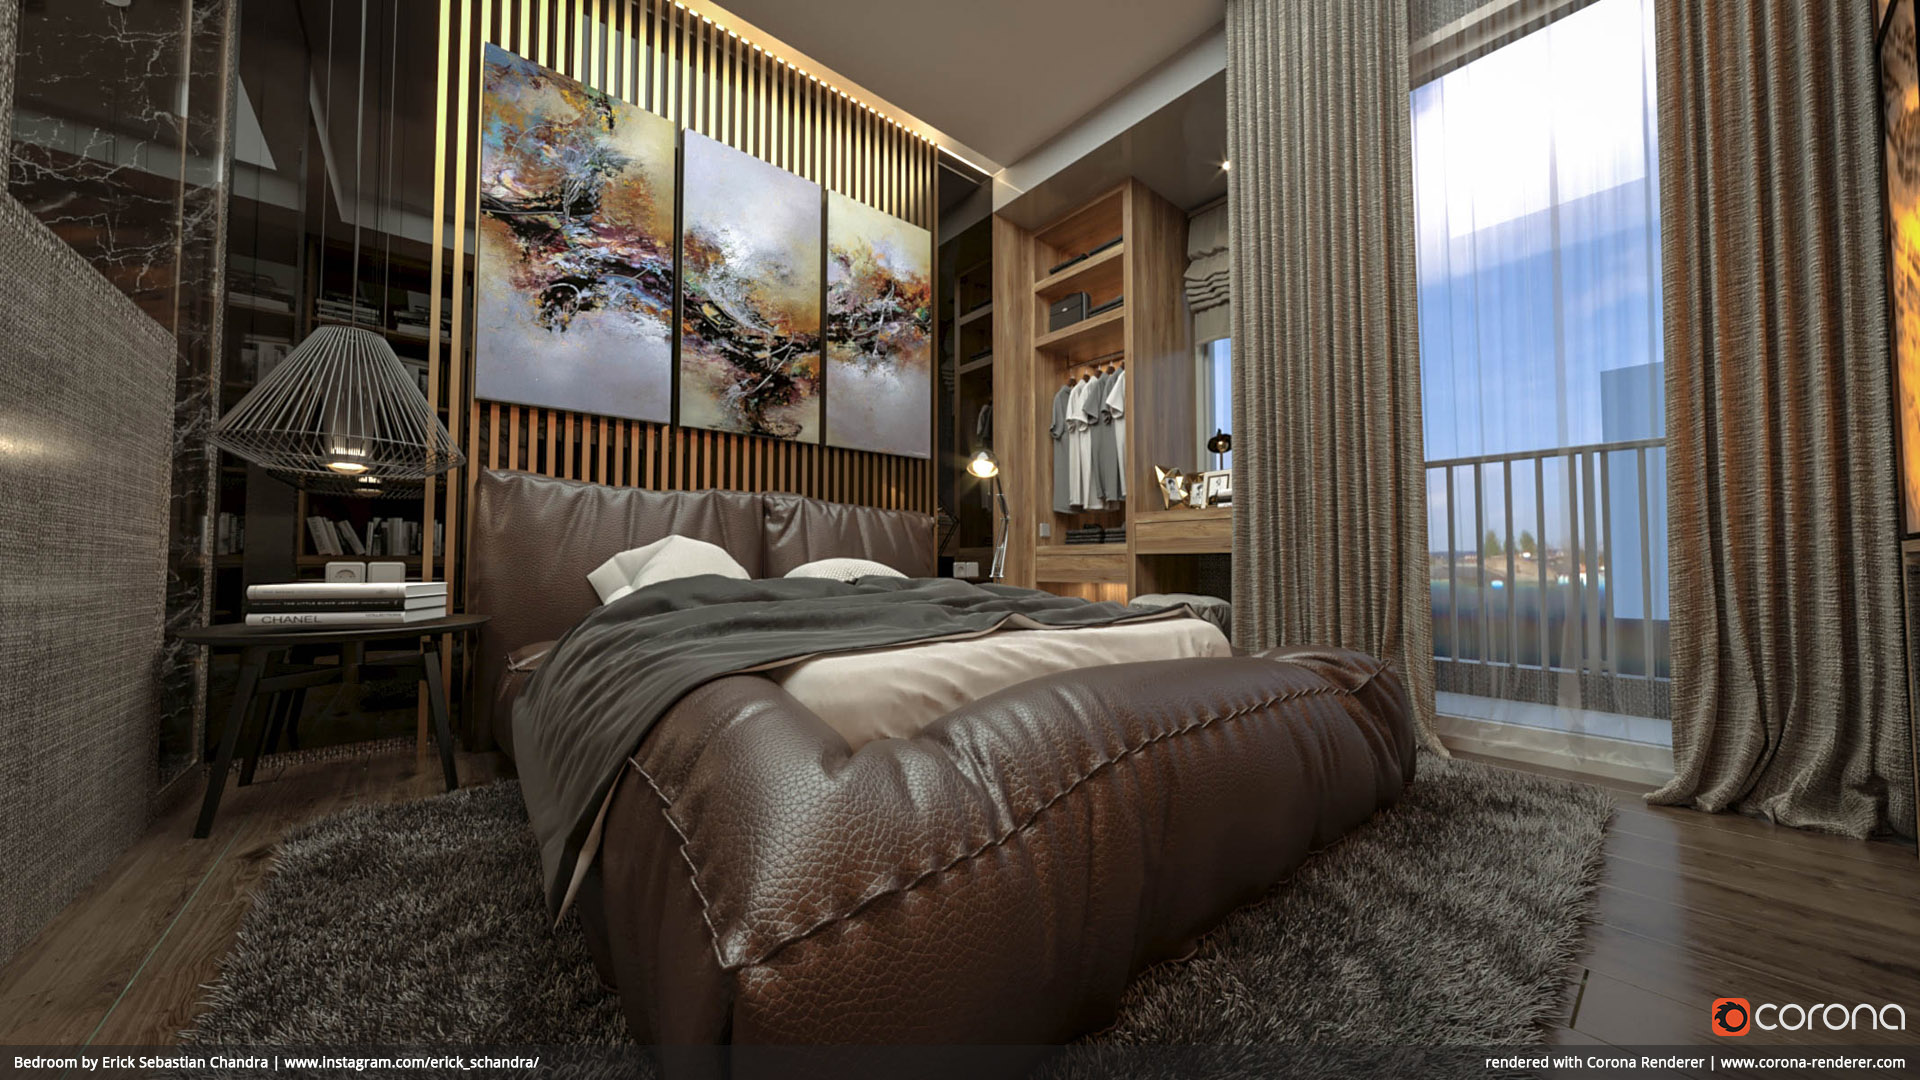
\includegraphics[width=\linewidth]{img/corona_render.jpg}
	\caption{An image generated with the Corona Renderer}
	\label{fig:corona_render}
\end{figure}

The main idea is similar for every renderer:
\begin{enumerate}
	\item A 3D digital scene is described by the objects it contains
	\item A light simulation algorithm runs for every visible pixel from the viewer
	\item Upon object interaction, the shading of the intersected point is computed
	\item When it's done, results in form of a picture ("photograph") called \emph{render} are created
\end{enumerate}

Please see figure ~\ref{fig:path_tracer} for a simple demonstration of this workflow.

\begin{figure}[H]
	\centering
	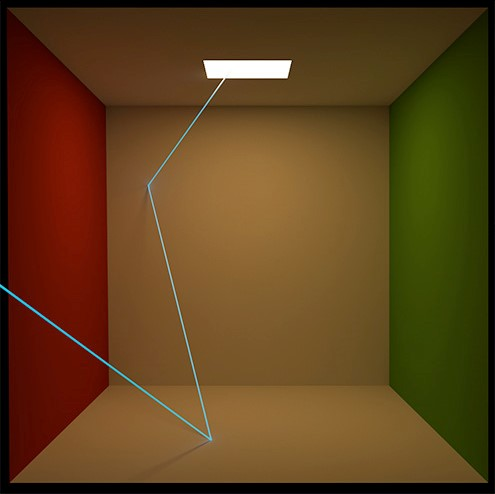
\includegraphics[width=85mm]{img/path_tracer.jpg}
	\caption{A visualization of a light transport algorithm (path tracer)~\cite{mitsubaWeb}}
	\label{fig:path_tracer}
\end{figure}

\subsection{Digital scene}

The basic elements of a digital scene are roughly the same for each renderer. 

\begin{description}
	\item[Camera] A camera in a digital scene works in the same manner as in real life --- it records a picture. Generally, you may define the coordinate position and the viewing vectors but also the properties such as focal distance or the type of film.
	\item[Light source] The scene needs to be illuminated by one or multiple sources in order to be visible. The common kinds of lights are point light, area light, spot light or environment (constant) lighting. 
	\item[Objects] The actual visible content of the scene are objects. Almost all rendering systems offer a choice to either use their precomputed basic geometry such as spheres or triangles or to include a mesh geometry described in an external file (usually created by modeling software). They also have to state their material properties so that the algorithm may correctly interact with them, e.g. diffuse vs. reflective material.
\end{description}

Unfortunately, as each renderer may have a very unique implementation details, the formats of the scenes are vastly different. For example, mitsuba uses XML but PBRT has its own specific format. An example of a simple scene for Mitsuba2 can be found in \ref{fig:example_scene}.

\definecolor{maroon}{rgb}{0.5,0,0}
\definecolor{darkgreen}{rgb}{0,0.5,0}
\lstdefinelanguage{XML}
{
	basicstyle=\ttfamily,
	morestring=[s]{"}{"},
	morecomment=[s]{?}{?},
	morecomment=[s]{!--}{--},
	commentstyle=\color{darkgreen},
	moredelim=[s][\color{black}]{>}{<},
	moredelim=[s][\color{red}]{\ }{=},
	stringstyle=\color{blue},
	identifierstyle=\color{maroon}
}

\begin{figure}[httpb]
\begin{tabular}{p{0.3\textwidth}p{0.6\textwidth}}
\begin{minipage}{0.3\textwidth}
	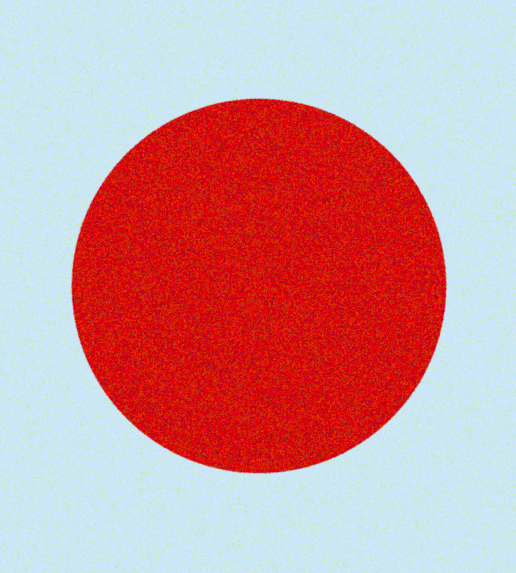
\includegraphics[width=\linewidth]{img/example_scene.png}
\end{minipage}
	&
\begin{minipage}{0.6\textwidth}
	\lstset{language=XML}
	\begin{lstlisting}[basicstyle=\tiny]
<scene version="2.0.0">
 <!-- Light transport algorithm -->
 <integrator type="path"/>
	
 <!-- Camera looking at the sphere -->
 <sensor type="perspective">
  <transform name="to_world">
   <lookat origin="0,-6,0" target="0,0,0" up="0,0,1"/>
  </transform>
 </sensor>
	
 <!-- Red sphere in the middle -->
 <shape type="sphere">
  <bsdf type="diffuse">
   <rgb name="reflectance" value="1.0,0.0,0.0"/>
  </bsdf>
 </shape>
	
 <!-- Light blue light all around the scene-->
 <emitter type="constant">
  <rgb name="radiance" value="0.6,0.8,0.9"/>
 </emitter>
</scene>
	\end{lstlisting}
\end{minipage}
\end{tabular}
\label{fig:example_scene}
\caption{A simple scene rendered with Mitsuba2 (left) along with its scene descriptiont (right)}
\end{figure}

\subsection{Light simulation}

The fundamental part of the rendering process is its implementation of the light transport simulation. The following sections will describe the theory and the physics models that are behind the light transport and then we look at the specific algorithms. 

\subsubsection{BRDF}

The materials of objects inside a scene are described by \emph{Bidirection Distrubtion Reflectance Function}, shortly \emph{BRDF}. This function is given the incoming vector $\omega_i$, the outgoing vector $\omega_o$ and it tells us how much radiance is reflected from the direction $\omega_i$ to the direction $\omega_o$. By the definition~\cite{nicodemus1965directional}, it looks as follows:

\begin{equation}
f_r(\omega_i,\omega_o)=\frac{dL_o(\omega_o)}{L_i(\omega_i)cos\theta_i d\omega_i}
\end{equation}

The function is shown in \ref{fig:brdf}. As it is a distribution function, we can rather describe it as a probability density that a defined amount of light energy gets reflected from $\omega_i$ to $\omega_o$.

\begin{figure}[H]
	\centering
	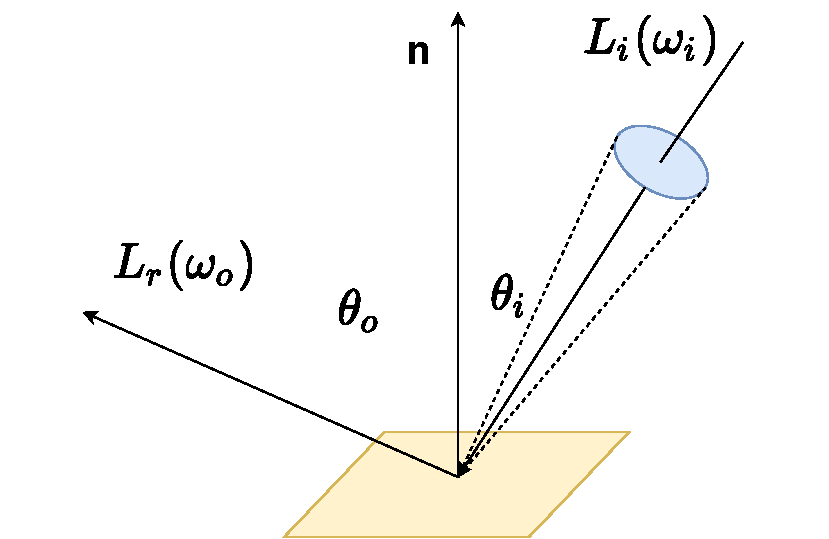
\includegraphics[width=85mm]{img/brdf.pdf}
	\caption{A Bidirectional Distribution Reflectance Function}
	\label{fig:brdf}
\end{figure}

In the simplest cases this states how reflective the surface of an object is. A comparison between diffuse and reflective BRDFs is displayed in 

\begin{figure}[H]
	\centering
	\begin{minipage}{.5\textwidth}
		\centering
		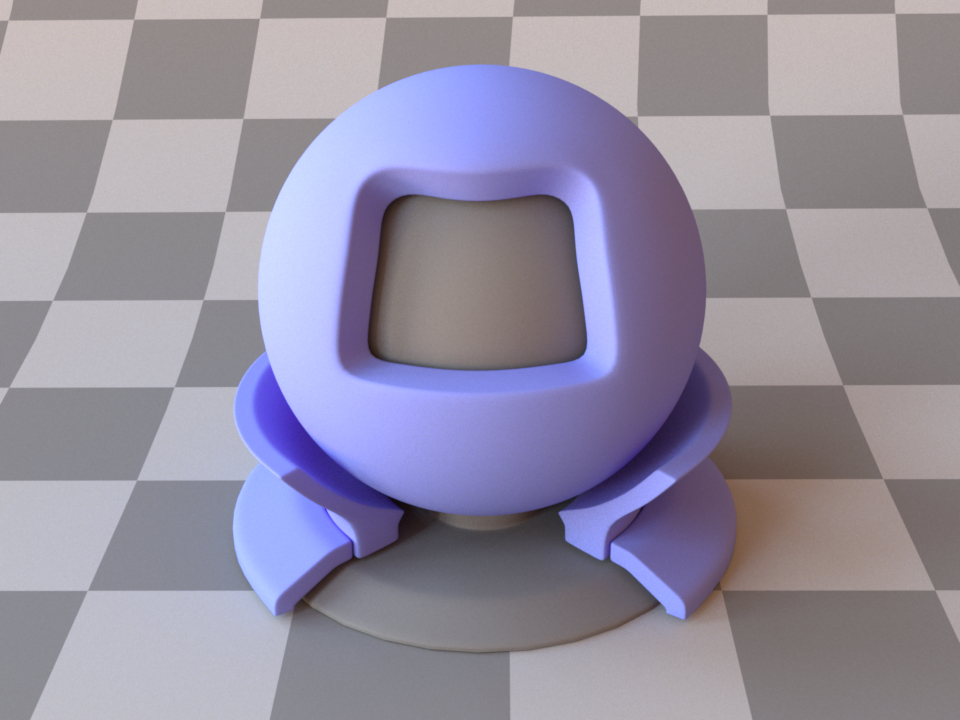
\includegraphics[width=.9\linewidth]{img/bsdf_diffuse.jpg}
	\end{minipage}%
	\begin{minipage}{.5\textwidth}
		\centering
		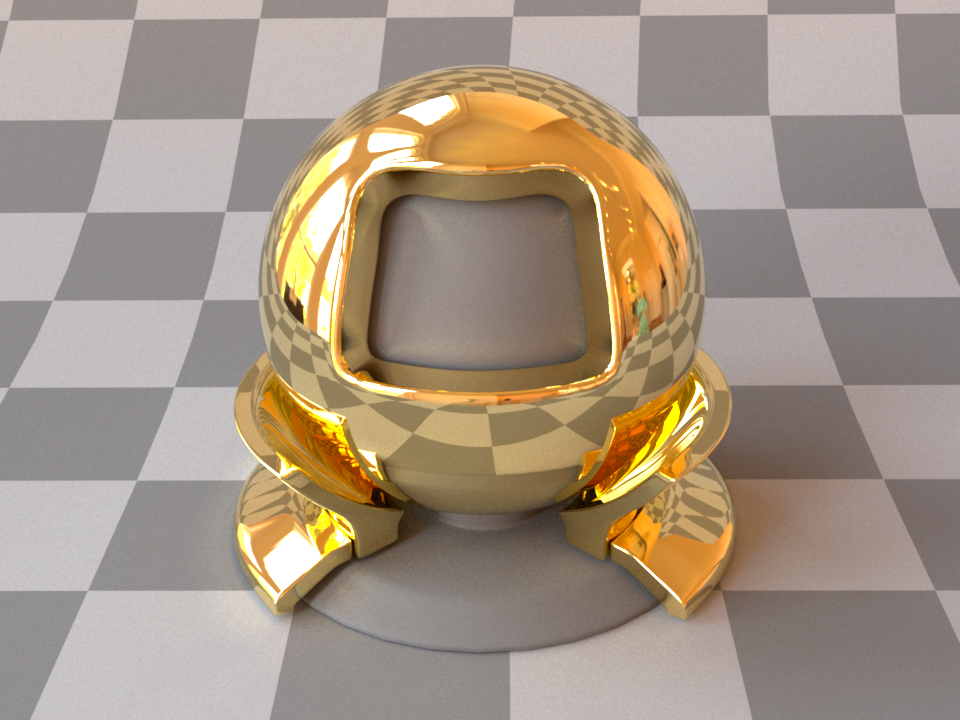
\includegraphics[width=.9\linewidth]{img/bsdf_reflective.jpg}
	\end{minipage}
\caption{Diffuse (left) and reflective gold (right) by Mitsuba2~\cite{mitsubaWeb}}
\label{fig:diffuse_reflective}
\end{figure}

Physically based BRDFs must fulfill several properties~\citealp{duvenhage2013numerical}:
\begin{description}
	\item[Heimholtz reciprocity] The amount of reflected energy from the incoming direction to the outgoing direction is equal to the amount of energy in the reversed directions ($f_r(\omega_i,\omega_o)=f_r(\omega_o,\omega_i)$)
	\item[Energy conservation] The amount of reflected energy cannot be larger than received
	\item[Positivity] BRDF is always positive ($f_r(\omega_i,\omega_o)\le0$)
\end{description}

Note that BRDF concerns only opaque surfaces. There exist multiple distribution functions that describe behavior of other materials, for example:
\begin{description}
	\item[BTDF] Describes light transmission
	\item[BSDF] Combination of BTDF and BRDF (e.g. glass, water)
	\item[BSSRDF] Considers scattering of the light under the surface as well (skin)
\end{description}


\subsubsection{Rendering equation}

The physically based realistic rendering is in reality an approach to solve some of the formulations of the \emph{rendering equation}~\cite{kajiya1986rendering}. It looks as follows:

\begin{equation}
L_o(x,\omega_o)=L_e(x,\omega_o)+\int_{\Omega}f_r(x,\omega_o,\omega_i) L_i(x,\omega_,i) cos\theta_i d\omega_i
\end{equation}





\chapter{Spectral Rendering}

\section{Color representation}

\section{Rendering process}

\section{Conversions to RGB}

\section{Advantages}

\section{Disadvantages}

\chapter{Appearance Computations}
\label{chap:appearance}

\section{Reflectance}

\section{Spectral accuracy}

\section{Polarization}

\section{Fluorescence}

\section{Iridescence}

\section{Dispersion}
\chapter{Supported Spectral Renderers}

\section{Mitsuba2}

\section{ART}
\chapter{Benchmark}

\section{Framework}

\section{Supported Spectral Renderers}

\subsection{Mitsuba2}

\subsection{ART}

\section{Scenes}

\subsection{GGX Reflectance}

\subsection{Spectral accuracy}

\subsection{Polarization}

\subsection{Fluorescence}

\section{Common Data}

\section{Usage}

\section{Open source contributions}

\subsection{GGX for ART}

\subsection{Iridescence for Mitsuba2}

\subsection{Multi-channel EXR support for jeri.io}

\section{Future Work}

\chapter*{Conclusion}
\addcontentsline{toc}{chapter}{Conclusion}


%%% Bibliography
%%% Bibliography (literature used as a source)
%%%
%%% We employ bibTeX to construct the bibliography. It processes
%%% citations in the text (e.g., the \cite{...} macro) and looks up
%%% relevant entries in the bibliography.bib file.
%%%
%%% The \bibliographystyle command selects, which style will be used
%%% for references from the text. The argument in curly brackets is
%%% the name of the corresponding style file (*.bst). Both styles
%%% mentioned in this template are included in LaTeX distributions.

\bibliographystyle{plainnat}    %% Author (year)
% \bibliographystyle{unsrt}     %% [number]

\renewcommand{\bibname}{Bibliography}

%%% Generate the bibliography. Beware that if you cited no works,
%%% the empty list will be omitted completely.

\bibliography{bibliography}

%%% If case you prefer to write the bibliography manually (without bibTeX),
%%% you can use the following. Please follow the ISO 690 standard and
%%% citation conventions of your field of research.

% \begin{thebibliography}{99}
%
% \bibitem{lamport94}
%   {\sc Lamport,} Leslie.
%   \emph{\LaTeX: A Document Preparation System}.
%   2nd edition.
%   Massachusetts: Addison Wesley, 1994.
%   ISBN 0-201-52983-1.
%
% \end{thebibliography}


%%% Figures used in the thesis (consider if this is needed)
%%%\listoffigures

%%% Tables used in the thesis (consider if this is needed)
%%% In mathematical theses, it could be better to move the list of tables to the beginning of the thesis.
%%%\listoftables

%%% Abbreviations used in the thesis, if any, including their explanation
%%% In mathematical theses, it could be better to move the list of abbreviations to the beginning of the thesis.
%%%\chapwithtoc{List of Abbreviations}

%%% Attachments to the master thesis, if any. Each attachment must be
%%% referred to at least once from the text of the thesis. Attachments
%%% are numbered.
%%%
%%% The printed version should preferably contain attachments, which can be
%%% read (additional tables and charts, supplementary text, examples of
%%% program output, etc.). The electronic version is more suited for attachments
%%% which will likely be used in an electronic form rather than read (program
%%% source code, data files, interactive charts, etc.). Electronic attachments
%%% should be uploaded to SIS and optionally also included in the thesis on a~CD/DVD.
%%% Allowed file formats are specified in provision of the rector no. 72/2017.
%%%\appendix
%%%\chapter{Attachments}

%%%\section{First Attachment}

\openright
\end{document}
